\begin{figure}[!t]
\centering
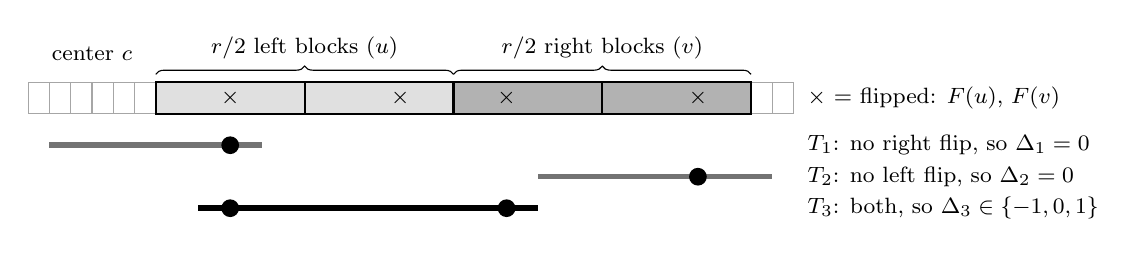
\begin{tikzpicture}[x=0.27cm,y=0.40cm,font=\footnotesize]
 \foreach \x in {0,...,35} \draw[black!35] (\x,0) rectangle ++(1,1);
 \fill[black!12] (6,0) rectangle (13,1);  \fill[black!12] (13,0) rectangle (20,1);
 \fill[black!30] (20,0) rectangle (27,1); \fill[black!30] (27,0) rectangle (34,1);
 \foreach \a in {6,13,20,27} \draw[thick] (\a,0) rectangle ++(7,1);
 \draw[decorate,decoration={brace,amplitude=3pt}] (6,1.25) -- (20,1.25) node[midway,above=2pt]{$r/2$ left blocks ($u$)};
 \draw[decorate,decoration={brace,amplitude=3pt}] (20,1.25) -- (34,1.25) node[midway,above=2pt]{$r/2$ right blocks ($v$)};
 \node at (3,1.9) {center $c$};
 \node at (9.5,0.5) {$\times$};  \node at (17.5,0.5) {$\times$};
 \node at (22.5,0.5) {$\times$}; \node at (31.5,0.5) {$\times$};
 \node[anchor=west] at (36.2,0.5) {$\times$ = flipped: $F(u)$, $F(v)$};
 \draw[line width=2pt,black!55] (1,-1) -- (11,-1);   \node[anchor=west] at (36.2,-1) {$T_1$: no right flip, so $\Delta_1=0$};
 \draw[line width=2pt,black!55] (24,-2) -- (35,-2);  \node[anchor=west] at (36.2,-2) {$T_2$: no left flip, so $\Delta_2=0$};
 \draw[line width=2pt,black]    (8,-3) -- (24,-3);   \node[anchor=west] at (36.2,-3) {$T_3$: both, so $\Delta_3\in\{-1,0,1\}$};
 \foreach \x/\y in {9.5/-1,22.5/-3,9.5/-3,31.5/-2} \fill (\x,\y) circle (3.2pt);
\end{tikzpicture}

\caption{A product-star cell. The cell fixes a center $c$ and, in each of $r$ blocks of
$b=2^s-1$ coordinates, lets the point move within a Hamming-code star (no flip or one flip); the left
pattern $u$ uses $r/2$ blocks and the right pattern $v$ the other $r/2$. A gate contributes to the
mixed residual only if it reads a coordinate flipped by $u$ and one flipped by $v$.}
\label{fig:cell}
\end{figure}
